%%%%%%%%%%%%%%%%%%%%%%%%%%%%%%%%%%%%%%%%%
% Beamer Presentation
% LaTeX Template
% Version 2.0 (March 8, 2022)
%
% This template originates from:
% https://www.LaTeXTemplates.com
%
% Author:
% Vel (vel@latextemplates.com)
%
% License:
% CC BY-NC-SA 4.0 (https://creativecommons.org/licenses/by-nc-sa/4.0/)
%
%%%%%%%%%%%%%%%%%%%%%%%%%%%%%%%%%%%%%%%%%

%----------------------------------------------------------------------------------------
%	PACKAGES AND OTHER DOCUMENT CONFIGURATIONS
%----------------------------------------------------------------------------------------

\documentclass[
	10pt, % Set the default font size, options include: 8pt, 9pt, 10pt, 11pt, 12pt, 14pt, 17pt, 20pt
	%t, % Uncomment to vertically align all slide content to the top of the slide, rather than the default centered
	aspectratio=169, % Uncomment to set the aspect ratio to a 16:9 ratio which matches the aspect ratio of 1080p and 4K screens and projectors
]{beamer}

\usepackage[all]{xy}

\usepackage[spanish]{babel}
\usepackage[utf8]{inputenc}

\graphicspath{{Images/}{./}} % Specifies where to look for included images (trailing slash required)

\usepackage{booktabs} % Allows the use of \toprule, \midrule and \bottomrule for better rules in tables

%\usepackage{tikz}
%\usetikzlibrary{positioning}
%\usetikzlibrary{shapes,arrows,arrows,positioning,fit}

\usepackage{tikz}
\usetikzlibrary{mindmap}

\usepackage{multirow}

\usepackage{graphicx}
\usepackage{hyperref}

\usepackage{venndiagram}

\usepackage{xcolor,listings}
\usepackage{textcomp}
\usepackage{color}

\usepackage{enumitem}

\usepackage{array}

\definecolor{codegreen}{rgb}{0,0.6,0}
\definecolor{codegray}{rgb}{0.5,0.5,0.5}
\definecolor{codepurple}{HTML}{C42043}
\definecolor{backcolour}{HTML}{F2F2F2}
\definecolor{red}{HTML}{FF0000}
\definecolor{bookColor}{cmyk}{0,0,0,0.90}  
\color{bookColor}

\lstset{upquote=true}

\lstdefinestyle{mystyle}{
	backgroundcolor=\color{backcolour},   
	commentstyle=\color{codegreen},
	keywordstyle=\color{codepurple},
	numberstyle=\numberstyle,
	stringstyle=\color{codepurple},
	basicstyle=\footnotesize\ttfamily,
	breakatwhitespace=false,
	breaklines=true,
	captionpos=b,
	keepspaces=true,
	numbers=left,
	numbersep=10pt,
	showspaces=false,
	showstringspaces=false,
	showtabs=false,
}
\lstset{style=mystyle}

\newcommand\numberstyle[1]{%
	\footnotesize
	\color{codegray}%
	\ttfamily
	\ifnum#1<10 0\fi#1 |%
}


%----------------------------------------------------------------------------------------
%	SELECT LAYOUT THEME
%----------------------------------------------------------------------------------------

% Beamer comes with a number of default layout themes which change the colors and layouts of slides. Below is a list of all themes available, uncomment each in turn to see what they look like.

%\usetheme{default}
%\usetheme{AnnArbor}
%\usetheme{Antibes}
%\usetheme{Bergen}
%\usetheme{Berkeley}
%\usetheme{Berlin}
%\usetheme{Boadilla} % interesante
%\usetheme{CambridgeUS}
%\usetheme{Copenhagen}
%\usetheme{Darmstadt}
%\usetheme{Dresden}
%\usetheme{Frankfurt}
%\usetheme{Goettingen}
%\usetheme{Hannover}
%\usetheme{Ilmenau}
%\usetheme{JuanLesPins}
%\usetheme{Luebeck}
\usetheme{Madrid} % interesante
%\usetheme{Malmoe}
%\usetheme{Marburg}
%\usetheme{Montpellier}
%\usetheme{PaloAlto}
%\usetheme{Pittsburgh} % interesante
%\usetheme{Rochester} % interesante este
%\usetheme{Singapore}
%\usetheme{Szeged}
%\usetheme{Warsaw}

%----------------------------------------------------------------------------------------
%	SELECT COLOR THEME
%----------------------------------------------------------------------------------------

% Beamer comes with a number of color themes that can be applied to any layout theme to change its colors. Uncomment each of these in turn to see how they change the colors of your selected layout theme.

%\usecolortheme{albatross}
%\usecolortheme{beaver}
%\usecolortheme{beetle}
%\usecolortheme{crane}
%\usecolortheme{dolphin}
%\usecolortheme{dove}
%\usecolortheme{fly}
%\usecolortheme{lily}
%\usecolortheme{monarca}
%\usecolortheme{seagull}
%\usecolortheme{seahorse}
%\usecolortheme{spruce} % verde suave
%\usecolortheme{whale}
%\usecolortheme{wolverine}

%----------------------------------------------------------------------------------------
%	SELECT FONT THEME & FONTS
%----------------------------------------------------------------------------------------

% Beamer comes with several font themes to easily change the fonts used in various parts of the presentation. Review the comments beside each one to decide if you would like to use it. Note that additional options can be specified for several of these font themes, consult the beamer documentation for more information.

\usefonttheme{default} % Typeset using the default sans serif font
%\usefonttheme{serif} % Typeset using the default serif font (make sure a sans font isn't being set as the default font if you use this option!)
%\usefonttheme{structurebold} % Typeset important structure text (titles, headlines, footlines, sidebar, etc) in bold
%\usefonttheme{structureitalicserif} % Typeset important structure text (titles, headlines, footlines, sidebar, etc) in italic serif
%\usefonttheme{structuresmallcapsserif} % Typeset important structure text (titles, headlines, footlines, sidebar, etc) in small caps serif

%------------------------------------------------

%\usepackage{mathptmx} % Use the Times font for serif text
%\usepackage{palatino} % Use the Palatino font for serif text

\usepackage{helvet} % Use the Helvetica font for sans serif text
%\usepackage[default]{opensans} % Use the Open Sans font for sans serif text
%\usepackage[default]{FiraSans} % Use the Fira Sans font for sans serif text
\usepackage[default]{lato} % Use the Lato font for sans serif text

%----------------------------------------------------------------------------------------
%	SELECT INNER THEME
%----------------------------------------------------------------------------------------

% Inner themes change the styling of internal slide elements, for example: bullet points, blocks, bibliography entries, title pages, theorems, etc. Uncomment each theme in turn to see what changes it makes to your presentation.

%\useinnertheme{default}
\useinnertheme{circles}
%\useinnertheme{rectangles}
%\useinnertheme{rounded}
%\useinnertheme{inmargin}

%----------------------------------------------------------------------------------------
%	SELECT OUTER THEME
%----------------------------------------------------------------------------------------

% Outer themes change the overall layout of slides, such as: header and footer lines, sidebars and slide titles. Uncomment each theme in turn to see what changes it makes to your presentation.

%\useoutertheme{default}
%\useoutertheme{infolines}
%\useoutertheme{miniframes}
%\useoutertheme{smoothbars}
%\useoutertheme{sidebar}
%\useoutertheme{split}
%\useoutertheme{shadow}
%\useoutertheme{tree}
%\useoutertheme{smoothtree}

\setbeamertemplate{footline} % Uncomment this line to remove the footer line in all slides
%\setbeamertemplate{footline}[page number] % Uncomment this line to replace the footer line in all slides with a simple slide count

\setbeamertemplate{navigation symbols}{} % Uncomment this line to remove the navigation symbols from the bottom of all slides

%----------------------------------------------------------------------------------------
%	PRESENTATION INFORMATION
%----------------------------------------------------------------------------------------

\title[Short Title]{Bases de Datos I} % The short title in the optional parameter appears at the bottom of every slide, the full title in the main parameter is only on the title page

\subtitle{Lenguaje de Consulta de Datos} % Presentation subtitle, remove this command if a subtitle isn't required

\author{Lic. Carlos Le\'on Gonz\'alez \\ Dra.C. Lucina Garc\'ia Hern\'andez} % Presenter name(s), the optional parameter can contain a shortened version to appear on the bottom of every slide, while the main parameter will appear on the title slide

\institute[UC]{Facultad de Matem\'atica y Computaci\'on \\ Universidad de La Habana \\ \smallskip} % Your institution, the optional parameter can be used for the institution shorthand and will appear on the bottom of every slide after author names, while the required parameter is used on the title slide and can include your email address or additional information on separate lines

\date[\today]{\today} % Presentation date or conference/meeting name, the optional parameter can contain a shortened version to appear on the bottom of every slide, while the required parameter value is output to the title slide

%----------------------------------------------------------------------------------------

\begin{document}

\lstset{
	literate=%
	{á}{{\'a}}1
	{í}{{\'i}}1
	{é}{{\'e}}1
	{ý}{{\'y}}1
	{ú}{{\'u}}1
	{ó}{{\'o}}1
	{ě}{{\v{e}}}1
	{š}{{\v{s}}}1
	{č}{{\v{c}}}1
	{ř}{{\v{r}}}1
	{ž}{{\v{z}}}1
	{ď}{{\v{d}}}1
	{ť}{{\v{t}}}1
	{ň}{{\v{n}}}1                
	{ů}{{\r{u}}}1
	{Á}{{\'A}}1
	{Í}{{\'I}}1
	{É}{{\'E}}1
	{Ý}{{\'Y}}1
	{Ú}{{\'U}}1
	{Ó}{{\'O}}1
	{Ě}{{\v{E}}}1
	{Š}{{\v{S}}}1
	{Č}{{\v{C}}}1
	{Ř}{{\v{R}}}1
	{Ž}{{\v{Z}}}1
	{Ď}{{\v{D}}}1
	{Ť}{{\v{T}}}1
	{Ň}{{\v{N}}}1                
	{Ů}{{\r{U}}}1    
}

%----------------------------------------------------------------------------------------
%	TITLE SLIDE
%----------------------------------------------------------------------------------------

\begin{frame}
	\titlepage % Output the title slide, automatically created using the text entered in the PRESENTATION INFORMATION block above
\end{frame}

%------------------------------------------------

\begin{frame}{t}
	
	\frametitle{¿Qué es lo mínimo a implementar en una BD?}
	
	\only<2>{
		\begin{center}
			CRUD
		\end{center}
		}
	
	\only<3>{
		\hspace{10em} \textbf{C} reate \ \ \ (Insert)
	
		\hspace{10em} \textbf{R} ead \ \ \ \ \ \ (\textcolor{red}{Select})  
	
		\hspace{10em} \textbf{U} pdate \ \ (Update)
	
		\hspace{10em} \textbf{D} elete \ \ \ (Delete)
	}

\end{frame}

%------------------------------------------------

\begin{frame}{t}
	
	\frametitle{Definiendo las tablas}
	
	\begin{figure}[h]
	\centering
		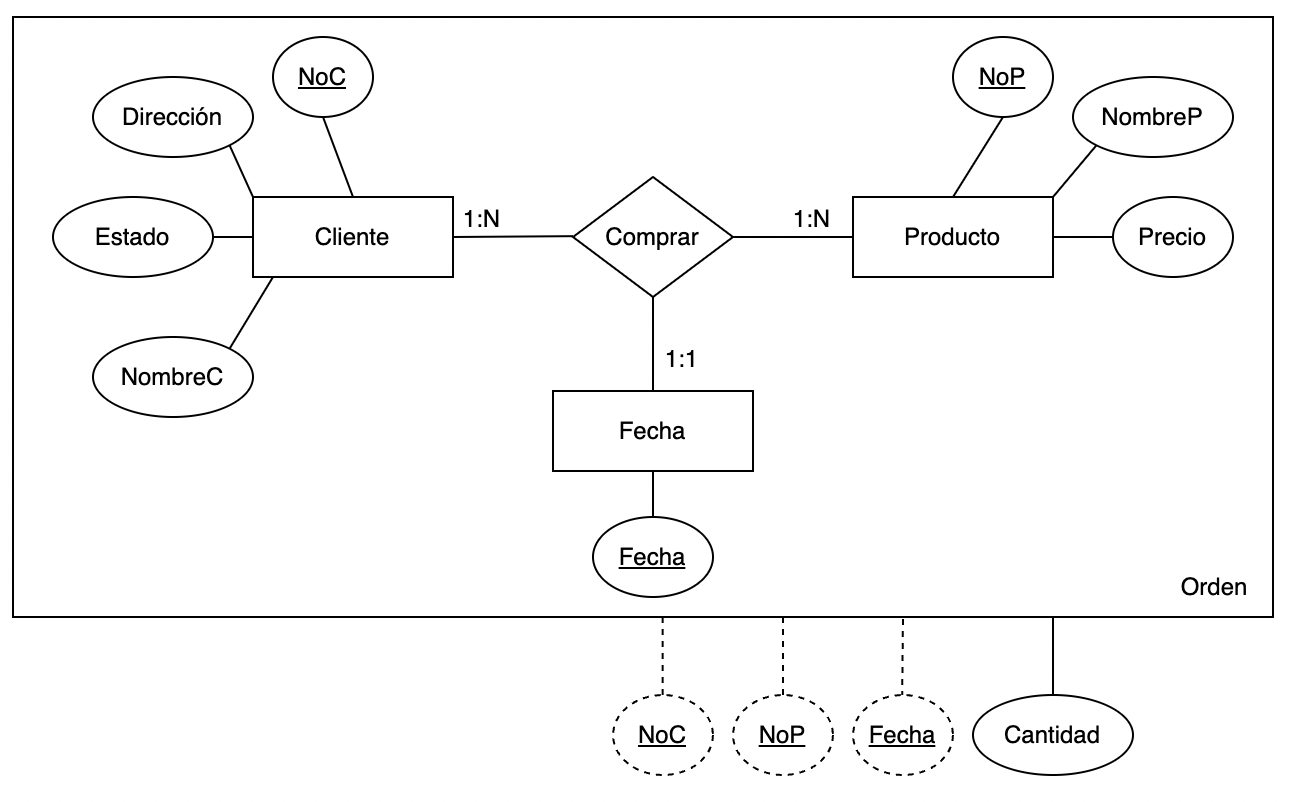
\includegraphics[scale=0.5]{bd.png}
	\end{figure}

	
\end{frame}

%------------------------------------------------

\begin{frame}[fragile]
	
	\frametitle{Iniciando con la sintaxis de la cláusula SELECT}
	
		\begin{lstlisting}[ language=SQL,
			deletekeywords={IDENTITY},
			deletekeywords={[2]INT},
			morekeywords={clustered},
			framesep=8pt,
			xleftmargin=40pt,
			framexleftmargin=40pt,
			frame=tb,
			framerule=0pt ]
SELECT * | <column_1>, <column_2>, ...
FROM <table_name>;
\end{lstlisting}

	\pause
	
	\ 
	
	\ 
	
	\begin{itemize}[label={}]
		\item SELECT: Define columnas a tomar
		\item FROM: Define la tabla a consultar
	\end{itemize}

\end{frame}

%------------------------------------------------

\begin{frame}[fragile]
	
	\frametitle{La primera consulta}
	
	Sintaxis:
	\begin{lstlisting}[ language=SQL,
		deletekeywords={IDENTITY},
		deletekeywords={[2]INT},
		morekeywords={clustered},
		framesep=8pt,
		xleftmargin=40pt,
		framexleftmargin=40pt,
		frame=tb,
		framerule=0pt ]
SELECT * | <column_1>, <column_2>, ...
FROM <table_name>;
\end{lstlisting}

	\ 
	
	\  
	
		
	Construya una consulta para ver la información del \textbf{cliente}.
	
	\pause

	\begin{columns}[t]
		\column{0.5\textwidth}
		\begin{lstlisting}[ language=SQL,
			deletekeywords={IDENTITY},
			deletekeywords={[2]INT},
			morekeywords={clustered},
			framesep=8pt,
			xleftmargin=40pt,
			framexleftmargin=40pt,
			frame=tb,
			framerule=0pt ]
SELECT *
FROM cliente;
\end{lstlisting}
	
	\column{0.5\textwidth}
	
		\begin{lstlisting}[ language=SQL,
		deletekeywords={IDENTITY},
		deletekeywords={[2]INT},
		morekeywords={clustered},
		framesep=8pt,
		xleftmargin=40pt,
		framexleftmargin=40pt,
		frame=tb,
		framerule=0pt ]
SELECT NoC, NombreC, Dirección, Estado
FROM cliente;
\end{lstlisting}
	
	\end{columns}
	
	\pause
	
	\ 
	
	Dos consultas que generan el mismo resutado, pero una aprovecha el ``azúcar'' sintáctica de SQL.
	
	\pause
	
	\ 
	
	\textcolor{codepurple}{¿Cómo elegir las filas a mostrar?}
			
\end{frame}

%------------------------------------------------

\begin{frame}[fragile]
	
	\frametitle{Seleccionando filas}
	
	Sintaxis:
	\begin{lstlisting}[ language=SQL,
		deletekeywords={IDENTITY},
		deletekeywords={[2]INT},
		morekeywords={clustered},
		framesep=8pt,
		xleftmargin=40pt,
		framexleftmargin=40pt,
		frame=tb,
		framerule=0pt ]
SELECT * | <column_1>, <column_2>, ...
FROM <table_name>
WHERE <constraint_expresion>;
\end{lstlisting}

	\ 
	
	\pause 
	
	Posibles operadores a usar: 
	\begin{itemize}
	
		\item Lógicos: $AND$, $OR$, $NOT$
		
		\item Relacionales: $<$, $<=$, $>=$, $>$, $=$, $<>$
		
		
		\pause
		
		\ 
		
		Construya una consulta para obtener todos los productos cuyo precio sea menor o igual a $10$, o mayor que $2000$.
		
		\pause
		
		\ 
			\begin{lstlisting}[ language=SQL,
			deletekeywords={IDENTITY},
			deletekeywords={[2]INT},
			morekeywords={clustered},
			framesep=8pt,
			xleftmargin=40pt,
			framexleftmargin=40pt,
			frame=tb,
			framerule=0pt ]
SELECT NombreP, Precio
FROM producto
WHERE Precio <= 10 OR Precio > 2000; 
\end{lstlisting}
		
	\end{itemize}
	
\end{frame}

%------------------------------------------------

\begin{frame}[fragile]
	
	\frametitle{Seleccionando filas}
	
	Sintaxis:
	\begin{lstlisting}[ language=SQL,
		deletekeywords={IDENTITY},
		deletekeywords={[2]INT},
		morekeywords={clustered},
		framesep=8pt,
		xleftmargin=40pt,
		framexleftmargin=40pt,
		frame=tb,
		framerule=0pt ]
SELECT expresion
FROM table_name
WHERE constraint_expresion;
\end{lstlisting} 
	
	Posibles operadores a usar: 
	\begin{itemize}
		
		\item Especiales: $IN$, $LIKE$, $BETWEEN$, $IS\ NULL$
		
		\pause 
		
		\ 
		
		Construya una consulta para obtener todos los clientes que pertenezcan a ``Ohio'', ``Nevada'' o ``Misisipi''.
		
		\pause
		
		\begin{columns}[t]
			\column{0.5\textwidth}
			\begin{lstlisting}[ language=SQL,
				deletekeywords={IDENTITY},
				deletekeywords={[2]INT},
				morekeywords={clustered},
				framesep=8pt,
				xleftmargin=40pt,
				framexleftmargin=40pt,
				frame=tb,
				framerule=0pt ]
SELECT NombreC 
FROM cliente 
WHERE Estado IN ('Ohio', 'Nevada', 'Misisipi');
\end{lstlisting}
			
			\column{0.5\textwidth}
			\begin{lstlisting}[ language=SQL,
				deletekeywords={IDENTITY},
				deletekeywords={[2]INT},
				morekeywords={clustered},
				framesep=8pt,
				xleftmargin=40pt,
				framexleftmargin=40pt,
				frame=tb,
				framerule=0pt ]
SELECT NombreC 
FROM cliente 
WHERE Estado = 'Ohio' OR  Estado = 'Nevada' OR Estado =  'Misisipi';
\end{lstlisting}
			
		\end{columns}
		
	\end{itemize}
	
\end{frame}

%------------------------------------------------

\begin{frame}[fragile]
	
	\frametitle{Seleccionando filas}
	
	Sintaxis:
	\begin{lstlisting}[ language=SQL,
		deletekeywords={IDENTITY},
		deletekeywords={[2]INT},
		morekeywords={clustered},
		framesep=8pt,
		xleftmargin=40pt,
		framexleftmargin=40pt,
		frame=tb,
		framerule=0pt ]
SELECT <expresion>
FROM <table_name>
WHERE <constraint_expresion>;
\end{lstlisting} 
	
	Posibles operadores a usar: 
	\begin{itemize}
		
		\item Especiales: $IN$, $LIKE$, $BETWEEN$, $IS\ NULL$
		
		\pause 
		
		\ 
		
		Construya una consulta para obtener todos los clientes cuyo nombre comience con la letra ``\texttt{I}'' y culmine con al menos cuatro letras, donde las dos últimas tienen que ser ``\texttt{er}''. La columna de la tabla resultante tiene que llamarse ``Cliente Especial I-er''.
		
		\pause
		
			\begin{lstlisting}[ language=SQL,
				deletekeywords={IDENTITY},
				deletekeywords={[2]INT},
				morekeywords={clustered},
				framesep=8pt,
				xleftmargin=40pt,
				framexleftmargin=40pt,
				frame=tb,
				framerule=0pt ]
SELECT NombreC AS `Cliente Especial I-er`
FROM cliente 
WHERE NombreC LIKE 'I%_er';
\end{lstlisting}
			
	\end{itemize}
	
\end{frame}

%------------------------------------------------

\begin{frame}[fragile]
	
	\frametitle{Desglosando el comando LIKE}
	
			\begin{lstlisting}[ language=SQL,
			deletekeywords={IDENTITY},
			deletekeywords={[2]INT},
			morekeywords={clustered},
			framesep=8pt,
			xleftmargin=40pt,
			framexleftmargin=40pt,
			frame=tb,
			framerule=0pt ]
SELECT NombreC AS `Cliente Especial I-er`
FROM cliente 
WHERE NombreC LIKE 'I%_er';
\end{lstlisting}

	\ 
	
	\ 
	
	El comando \textcolor{codepurple}{AS} brinda alias a columnas o tablas.
	
	\pause
	
	\ 
	
	Comodines de  \textcolor{codepurple}{LIKE}: 
	\begin{itemize}
		
		\item \textcolor{codepurple}{$\%$} Representa cero, uno o múltiples caracteres
		
		\item \textcolor{codepurple}{\textbf{$\_$}} \ \ Representa un solo caracter
					
	\end{itemize}
	
	\pause 
	
	\ 
	
	Existen otros comodines que permiten generalizar el comando y utilizarlo con expresiones regulares.
	
	\pause
	
	\ 
	
	\textcolor{red}{¿Cómo ordenar la relación resultante?}
	
\end{frame}

%------------------------------------------------

\begin{frame}[fragile]

	\frametitle{Ordenando los resultados}
	
	Construya una consulta para obtener todos los clientes, su dirección y su estado, pero ordenados de forma descendente por la dirección y el estado al que pertenecen.
	
	\pause
	
	\ 
	
	Sintaxis:
	\begin{lstlisting}[ language=SQL,
		deletekeywords={IDENTITY},
		deletekeywords={[2]INT},
		morekeywords={clustered},
		framesep=8pt,
		xleftmargin=40pt,
		framexleftmargin=40pt,
		frame=tb,
		framerule=0pt ]
SELECT <expresion>
FROM <table_name>
ORDER BY <field> [ASC|DESC], ...;
\end{lstlisting} 

	\pause
	
	\ 
	
	Solución:
	\begin{columns}[t]
		\column{0.5\textwidth}
		\begin{lstlisting}[ language=SQL,
			deletekeywords={IDENTITY},
			deletekeywords={[2]INT},
			morekeywords={clustered},
			framesep=8pt,
			xleftmargin=40pt,
			framexleftmargin=40pt,
			frame=tb,
			framerule=0pt ]
SELECT NombreC, Dirección, Estado 
FROM cliente 
ORDER BY Estado ASC, Dirección DESC;
\end{lstlisting} 
		
		\column{0.5\textwidth}
		\begin{lstlisting}[ language=SQL,
			deletekeywords={IDENTITY},
			deletekeywords={[2]INT},
			morekeywords={clustered},
			framesep=8pt,
			xleftmargin=40pt,
			framexleftmargin=40pt,
			frame=tb,
			framerule=0pt ]
SELECT NombreC, Dirección, Estado 
FROM cliente 
ORDER BY Estado, Dirección DESC;
\end{lstlisting} 
		
	\end{columns}
	
	\pause 
	
	\ 
	
	
	\textcolor{codepurple}{¿Cómo limitar el número de filas mostradas?}
	
\end{frame}

%------------------------------------------------

\begin{frame}[fragile]
	
	\frametitle{Limitando la cantidad de filas a mostrar}
	
	Sintaxis:
	\begin{lstlisting}[ language=SQL,
		deletekeywords={IDENTITY},
		deletekeywords={[2]INT},
		morekeywords={clustered},
		framesep=8pt,
		xleftmargin=40pt,
		framexleftmargin=40pt,
		frame=tb,
		framerule=0pt ]
SELECT * | <column_1>, <column_2>, ...
FROM <table_name>
LIMIT <number>;
\end{lstlisting}
	
	\pause 
	
	\ 
	
	\ 
	
	Con la siguiente consulta, se muestran solo 10 filas 
	
	\begin{lstlisting}[ language=SQL,
		deletekeywords={IDENTITY},
		deletekeywords={[2]INT},
		morekeywords={clustered},
		framesep=8pt,
		xleftmargin=40pt,
		framexleftmargin=40pt,
		frame=tb,
		framerule=0pt ]
SELECT *
FROM cliente
LIMIT 10;
\end{lstlisting}
	
	\pause
	
	\ 
	
	\ 
	
	
	\textcolor{red}{¿Qué pasa si se quiere resumir la información?}
	

\end{frame}

%------------------------------------------------

\begin{frame}[fragile]

	\frametitle{Agrupando los resultados}
	
	Construya una consulta que muestre la cantidad de clientes por estado.
	
		\pause
	
	\ 
	
	Sintaxis:
	\begin{lstlisting}[ language=SQL,
		deletekeywords={IDENTITY},
		deletekeywords={[2]INT},
		morekeywords={clustered},
		framesep=8pt,
		xleftmargin=40pt,
		framexleftmargin=40pt,
		frame=tb,
		framerule=0pt ]
SELECT <expresion>
FROM <table_name>
GROUP BY <field_1> [, <field_2>, ...] ;
\end{lstlisting} 
	
	\pause
	
	\ 
	
	Solución:
		\begin{lstlisting}[ language=SQL,
		deletekeywords={IDENTITY},
		deletekeywords={[2]INT},
		morekeywords={clustered},
		framesep=8pt,
		xleftmargin=40pt,
		framexleftmargin=40pt,
		frame=tb,
		framerule=0pt ]
SELECT Estado, COUNT(NoC) AS Cantidad
FROM cliente 
GROUP BY Estado;
\end{lstlisting} 
	
\end{frame}

%------------------------------------------------

\begin{frame}[fragile]
	
	\frametitle{Funciones útiles para resumir}
	
	\begin{itemize}
		
		\item COUNT() : Cuenta la cantidad de registros
		
		\item MAX() : Determina el valor máximo para una atributo
		
		\item MIN() : Determina el valor mínimo para una atributo
		
		\item SUM() : Suma los valores de un atributo
		
		\item AVG() : Calcula el promedio de los valores de un atributo
		
	\end{itemize}
	
	\ 
	
	\ 
	
	\pause
	
	Las funciones a utilizar por el uso de la cláusula \textcolor{codepurple}{GROUP BY} requieren un conjunto de valores dado por el nombre del atributo. En el caso de \textbf{COUNT}, no es necesario la definición de un atributo, basta con el uso de ``\textbf{*}''.
	
	\ 
	
	\ 
	
	\pause
	
	\textcolor{red}{¿Y si se quiere seleccionar algunas tuplas, luego de agrupar?}
	
\end{frame}

%------------------------------------------------

\begin{frame}[fragile]

	\frametitle{Añadiendo condición al agrupar}

	Sintaxis:
	\begin{lstlisting}[ language=SQL,
		deletekeywords={IDENTITY},
		deletekeywords={[2]INT},
		morekeywords={clustered},
		framesep=8pt,
		xleftmargin=40pt,
		framexleftmargin=40pt,
		frame=tb,
		framerule=0pt ]
SELECT <expresion>
FROM <table_name>
GROUP BY <field_1> [, <field_2>, ...]
HAVING <constraint_expresion>;
\end{lstlisting}

	\pause 

	\ 

	\  

	Construya una consulta que muestre la cantidad de clientes por estado tal que su total sea menor que 5. 

	\  

	\pause 

	\begin{lstlisting}[ language=SQL,
		deletekeywords={IDENTITY},
		deletekeywords={[2]INT},
		morekeywords={clustered},
		framesep=8pt,
		xleftmargin=40pt,
		framexleftmargin=40pt,
		frame=tb,
		framerule=0pt ]
al
\end{lstlisting}

	\pause
	
	\ 
	
	\textcolor{red}{Y si se quieren expresar alternativas, ¿qué cláusula me lo facilita?}

\end{frame}

%------------------------------------------------

\begin{frame}[fragile]
	
	\frametitle{Utilizando alternativas}
	
	La clásula  \textcolor{codepurple}{CASE} tiene un comportamiento similar al conocido \emph{if-then-else}. En caso de no tener definido ``else'' y no cumplirse ninguna condición, el retorno será \textbf{NULL}.
	
	\ 
	
	Sintaxis: 
	
	\begin{lstlisting}[ language=SQL,
		deletekeywords={IDENTITY},
		deletekeywords={[2]INT},
		morekeywords={clustered},
		framesep=8pt,
		xleftmargin=40pt,
		framexleftmargin=40pt,
		frame=tb,
		framerule=0pt ]
CASE
  WHEN condition_1 THEN result_1
  [WHEN condition_2 THEN result_2, 
  ...
  ELSE result]
END;
\end{lstlisting}
	
	\pause
	
	\ 
	
	Construya una consulta para conocer si el precio de un producto es barato, normal, caro o muy caro. 
	
	\begin{columns}[t]
		\column{0.5\textwidth}
			\begin{table}[]
				\begin{tabular}{|l|l|}
					\hline
					Etiqueta & Rango de precio \\ \hline \hline
					barato   & {[}0, 100)        \\ \hline
					normal   & {[}100, 1000)       \\ \hline
				\end{tabular}
			\end{table}
		
		\column{0.5\textwidth}
		
		\begin{table}[]
			\begin{tabular}{|l|l|}
				\hline
				Etiqueta   & Rango de precio \\ \hline \hline
				caro          & {[}1000, 2000)        \\ \hline
				muy caro & e.o.c       \\ \hline
			\end{tabular}
		\end{table}

	\end{columns}
	
	
\end{frame}

%------------------------------------------------

\begin{frame}[fragile]
	
	\frametitle{Utilizando \emph{if-then-else}}
	
	Construya una consulta para conocer si el precio de un producto es barato, normal, caro o muy caro. 
	
	\begin{columns}[t]
		\column{0.5\textwidth}
		\begin{table}[]
			\begin{tabular}{|l|l|}
				\hline
				Etiqueta & Rango de precio \\ \hline \hline
				barato   & {[}0, 100)        \\ \hline
				normal   & {[}100, 1000)       \\ \hline
			\end{tabular}
		\end{table}
		
		\column{0.5\textwidth}
		
		\begin{table}[]
			\begin{tabular}{|l|l|}
				\hline
				Etiqueta   & Rango de precio \\ \hline \hline
				caro          & {[}1000, 2000)        \\ \hline
				muy caro & e.o.c       \\ \hline
			\end{tabular}
		\end{table}
		
	\end{columns}
	
	\pause
	
	\ 
	
	\ 
	
	\begin{lstlisting}[ language=SQL,
		deletekeywords={IDENTITY},
		deletekeywords={[2]INT},
		morekeywords={clustered},
		framesep=8pt,
		xleftmargin=40pt,
		framexleftmargin=40pt,
		frame=tb,
		framerule=0pt ]
SELECT 
  NombreP as Producto, 
  CASE 
    WHEN Precio >= 0 AND Precio < 100 THEN 'barato'
    WHEN Precio >= 100 AND Precio < 1000 THEN 'normal'
    WHEN Precio >= 1000 AND Precio < 2000 THEN 'caro'
    ELSE 'muy caro'
  END AS `Tipo de precio`
FROM producto;
\end{lstlisting}
	
\end{frame}

%------------------------------------------------

{
	\setbeamertemplate{background canvas}
	{%
		
\includegraphics[width=\paperwidth,height=\paperheight]{sql_on_fire.jpg}
	}
	
	\begin{frame}
	\end{frame}
}

%------------------------------------------------

\begin{frame}{t}
	
	\frametitle{Recordando las tablas}
	
	\begin{figure}[h]
		\centering
		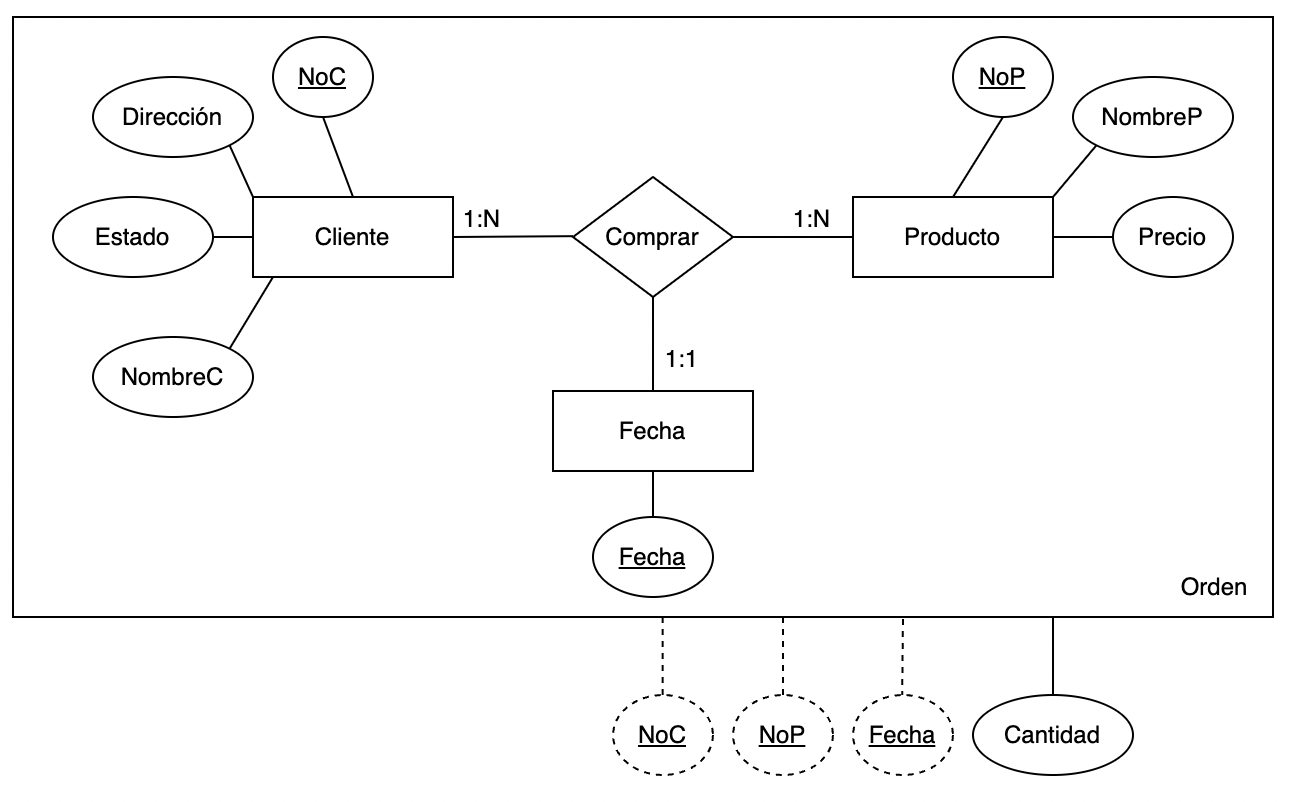
\includegraphics[scale=0.5]{bd.png}
	\end{figure}
	
	
\end{frame}

%------------------------------------------------

\begin{frame}[fragile]
	
		\frametitle{Vinculando tablas}
		
		La cláusula \textcolor{codepurple}{JOIN} permite relacionar varias tablas, usando las \emph{llaves foráneas} o bien columnas de referencias.
		
		\ 
		
		\ 
		
		\pause
		
		Sintaxis: 
		\begin{lstlisting}[ language=SQL,
			deletekeywords={IDENTITY},
			deletekeywords={[2]INT},
			morekeywords={clustered},
			framesep=8pt,
			xleftmargin=40pt,
			framexleftmargin=40pt,
			frame=tb,
			framerule=0pt ]
SELECT <expresion>
FROM <table_name_1>
  JOIN <table_name_2>
  ON <table_name_1>.<field_1> = <table_name_2>.<field_2>;
\end{lstlisting}
		
\end{frame}

%------------------------------------------------

\begin{frame}[fragile]
	
	\frametitle{Tipos de vínculos}
	
	\begin{center}
		
		\textcolor{codepurple}{INNER JOIN}
		
		\ 
		
		Obtiene todos los registros, siempre y cuando exista una coincidencia de los valores de las columnas definidas de ambas tablas.
		
		\begin{venndiagram2sets}[
			labelA={ }, labelOnlyA={Tabla1}, 
			labelB={ }, labelOnlyB={Tabla2}, 
			showframe=false]
			\fillACapB
		\end{venndiagram2sets}
		
	\end{center}
	
\end{frame}

%------------------------------------------------

\begin{frame}[fragile]
	
	\frametitle{Tipos de vínculos}
	
	\begin{center}
		\textcolor{codepurple}{INNER JOIN}
	\end{center}
	
	\ 
		
	Construya una consulta que muestre el cliente y la fecha en que efectuó alguna compra.
		
		\pause 
		
		\ 
		
		\ 
		
		\begin{lstlisting}[ language=SQL,
			deletekeywords={IDENTITY},
			deletekeywords={[2]INT},
			morekeywords={clustered},
			framesep=8pt,
			xleftmargin=40pt,
			framexleftmargin=40pt,
			frame=tb,
			framerule=0pt ]
SELECT 
  NombreC as Cliente, 
  Fecha
FROM orden 
  JOIN cliente
    ON orden.NoC = cliente.NoC;
\end{lstlisting}
				
\end{frame}

%------------------------------------------------

\begin{frame}[fragile]
	
	\frametitle{Tipos de vínculos}
	
	\begin{center}
	
		\textcolor{codepurple}{LEFT (OUTER) JOIN}
		
		\ 
		
		Obtiene todos los registros de la tabla que aparece en el \textcolor{codepurple}{FROM}, conocida como tabla izquierda (\textbf{Tabla1}). Los registros de la tabla posterior al \textcolor{codepurple}{JOIN}, conocida como tabla derecha (\textbf{Tabla2}), se añaden si existe alguna coincidencia de los valores de las columnas definidas. En caso contrario, se mostrará \textcolor{codepurple}{NULL}.
		
		\begin{venndiagram2sets}[
			labelA={ }, labelOnlyA={Tabla1}, 
			labelB={ }, labelOnlyB={Tabla2}, 
			showframe=false]
			\fillA
		\end{venndiagram2sets}
		
	\end{center}

\end{frame}
	
%------------------------------------------------

\begin{frame}[fragile]
	
	\frametitle{Tipos de vínculos}
	
	\begin{center}
		\textcolor{codepurple}{LEFT (OUTER) JOIN}
	\end{center}
	
	\ 
	
	Construya una consulta que muestre el cliente y la fecha en que efectuó alguna compra. Deben de aparecer también aquellos clientes que no hayan efectuado alguna compra.
	
	\pause 
	
	\ 
	
	\ 
	
	\begin{lstlisting}[ language=SQL,
		deletekeywords={IDENTITY},
		deletekeywords={[2]INT},
		morekeywords={clustered},
		framesep=8pt,
		xleftmargin=40pt,
		framexleftmargin=40pt,
		frame=tb,
		framerule=0pt ]
SELECT 
  NombreC AS Cliente, 
  Fecha
From cliente
  LEFT JOIN orden 
    ON orden.NoC = cliente.NoC;
\end{lstlisting}
	
\end{frame}

%------------------------------------------------

\begin{frame}[fragile]
	
	\frametitle{Tipos de vínculos}
	
	\begin{center}
	
		\textcolor{codepurple}{RIGHT (OUTER) JOIN}
		
		\ 
		
			Obtiene todos los registros de la tabla posterior al \textcolor{codepurple}{JOIN}, conocida como tabla derecha (\textbf{Tabla2}). Los registros de la tabla que aparece en el \textcolor{codepurple}{FROM}, conocida como tabla izquierda (\textbf{Tabla1}), se añaden si existe alguna coincidencia de los valores de las columnas definidas. En caso contrario, se mostrará \textcolor{codepurple}{NULL}.
		
		\begin{venndiagram2sets}[
			labelA={ }, labelOnlyA={Tabla1}, 
			labelB={ }, labelOnlyB={Tabla2}, 
			showframe=false]
			\fillB
		\end{venndiagram2sets}
		
	\end{center}
	
	\pause
	
	\ 
	
	\textcolor{red}{¿Qué devuelve la consulta anterior si se sustituye por el vínculo  \textcolor{codepurple}{RIGHT JOIN}?}
	
		
\end{frame}

%------------------------------------------------

\begin{frame}[fragile]
	
	\frametitle{Tipos de vínculos}		
	
	\begin{center}
	
		\textcolor{codepurple}{FULL (OUTER) JOIN}
		
		\ 
		
		Combina los resultados de los \emph{joins LEFT} y \emph{RIGHT}. Alternativamente, aparecerá \textcolor{codepurple}{NULL} cada registro de la tabla, cuando no haya coincidencia.		
		
		\begin{venndiagram2sets}[
			labelA={ }, labelOnlyA={Tabla1}, 
			labelB={ }, labelOnlyB={Tabla2}, 
			showframe=false]
			\fillA
			\fillB
		\end{venndiagram2sets}
	
	\end{center}
	
	\pause
	
	\ 
	
	\textcolor{red}{¿Qué devuelve la consulta anterior si se sustituye por el vínculo  \textcolor{codepurple}{FULL JOIN}?}
		
\end{frame}

%------------------------------------------------

\begin{frame}[fragile]
	
	\frametitle{¿Qué son las subconsultas?}
	
	\begin{itemize}
		
		\item En ocasiones, se necesita definir consultas anidadas, o sea, consultas dentro de otra consulta. Esto se conoce como \textbf{subconsultas}. 
		
		\item Las subconsultas pueden definirse en las cláusulas: \textcolor{codepurple}{SELECT}, \textcolor{codepurple}{FROM}, \textcolor{codepurple}{WHERE}, \textcolor{codepurple}{HAVING}.
		
		\item Existen reglas al utilizar subconsultas.
		
	\end{itemize}
		
\end{frame}

%------------------------------------------------

\begin{frame}[fragile]
	
	\frametitle{Trabajando con subconsultas}
	
	Construya una consulta para obtener los productos más baratos, teniendo en cuenta que: 
	
	\begin{columns}[t]
		\column{0.5\textwidth}
		\begin{table}[]
			\begin{tabular}{|l|l|}
				\hline
				Etiqueta & Rango de precio \\ \hline \hline
				barato   & {[}0, 100)        \\ \hline
				normal   & {[}100, 1000)       \\ \hline
			\end{tabular}
		\end{table}
		
		\column{0.5\textwidth}
		
		\begin{table}[]
			\begin{tabular}{|l|l|}
				\hline
				Etiqueta   & Rango de precio \\ \hline \hline
				caro          & {[}1000, 2000)        \\ \hline
				muy caro & e.o.c       \\ \hline
			\end{tabular}
		\end{table}
		
	\end{columns}
	
	\ 
	
	\pause
	
	\begin{lstlisting}[ language=SQL,
		deletekeywords={IDENTITY},
		deletekeywords={[2]INT},
		morekeywords={clustered},
		framesep=8pt,
		xleftmargin=40pt,
		framexleftmargin=40pt,
		frame=tb,
		framerule=0pt ]
SELECT Producto
From (
  SELECT 
    NombreP AS Producto, 
    CASE 
      WHEN Precio >= 0 AND Precio < 100 THEN 'barato'
      WHEN Precio >= 100 AND Precio < 1000 THEN 'normal'
      WHEN Precio >= 1000 AND Precio < 2000 THEN 'caro'
      ELSE 'muy caro'
    END AS `Tipo de precio`
  FROM producto
  ) AS table_tmp
WHERE `Tipo de precio` = 'barato';  
\end{lstlisting}
		
\end{frame}

%------------------------------------------------

\begin{frame}
	
	\begin{figure}[h]
		\centering
		
\includegraphics[scale=0.5]{mucho.png}
	\end{figure}
	
\end{frame}

%------------------------------------------------

\begin{frame}

	\frametitle{Orden de ejecución de las cláusulas}
	
	\begin{figure}[h]
		\centering
		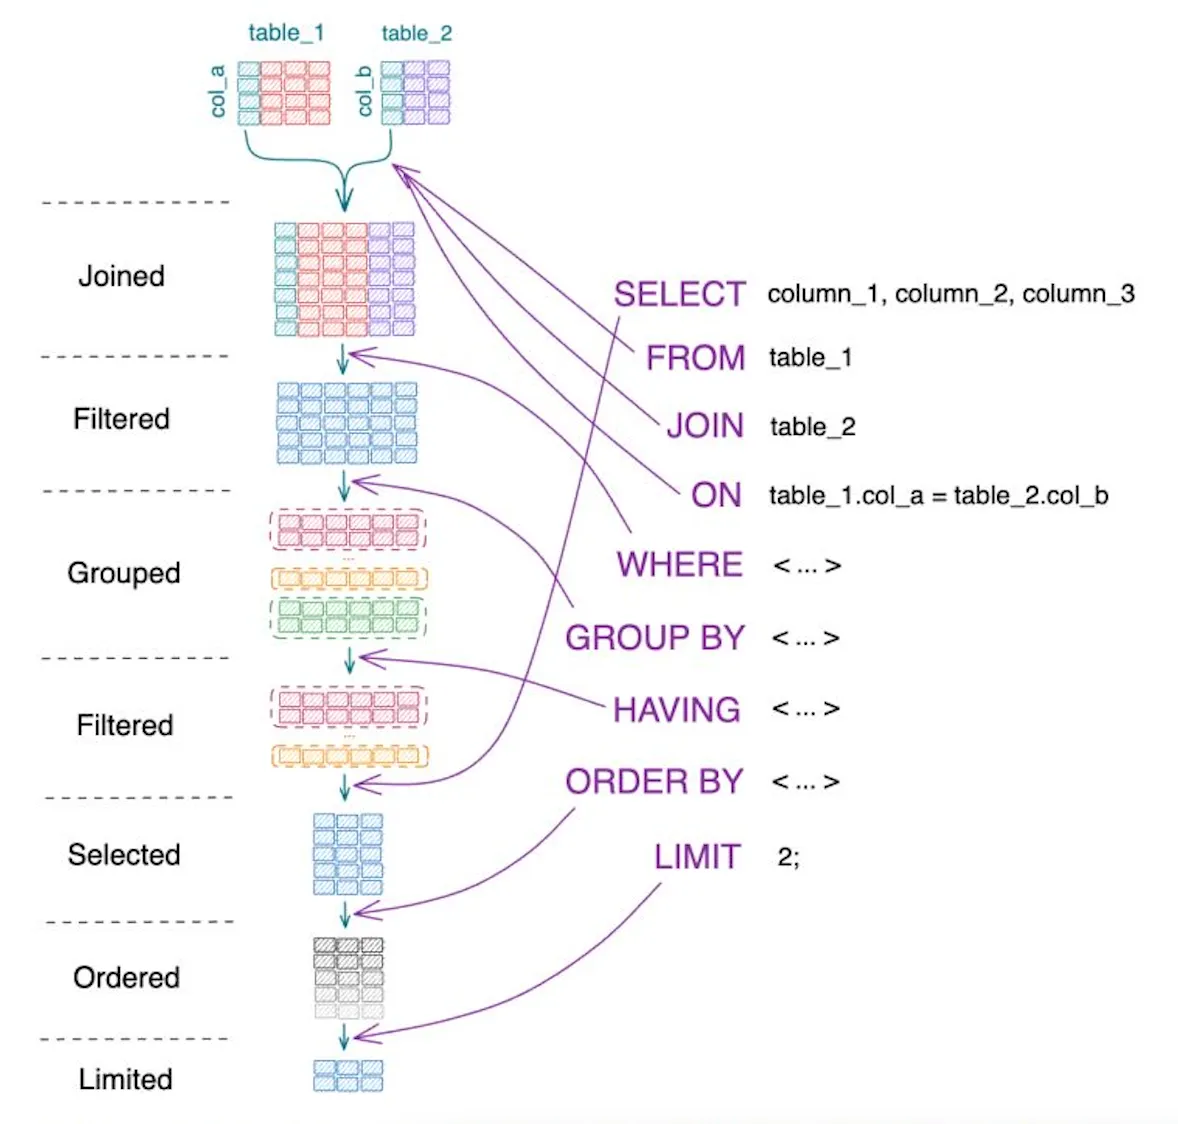
\includegraphics[scale=0.2]{orden.jpg}
	\end{figure}

\end{frame}

%------------------------------------------------

\begin{frame}
	
	\frametitle{Resumen de cláusulas}

\begin{table}[]
	\begin{tabular}{| l | c | m{6cm} | c |}
		\hline 
		Cláusula & \multicolumn{1}{l|}{¿Es obligatoria?} & ¿Qué hace? & \multicolumn{1}{l|}{¿Qué modifica?} \\ \hline \hline
		Select & Sí & Identifica las columnas a mostrar en la relación & - \\ \hline
		From & Sí & Determina la fuente de datos & - \\ \hline
		Where & No & Restringe los registros de la fuente de datos a utilizar & From (y Join) \\ \hline
		Join & No & Determina otras fuentes de datos y cómo relacionarlas con la establecida en el From & - \\ \hline
		Group By & No & Agrupa los registros ``similares''& - \\ \hline
		Having & No & Restringe los grupos & Group By \\ \hline
		Order by & No & Ordena los registros & - \\ \hline
		Limit & No & Limita la cantidad de registros a mostrar & - \\ \hline
	\end{tabular}
\end{table}




\end{frame}

%------------------------------------------------

\begin{frame}
	
	\frametitle{Dudas, preguntas, sugerencias ...}
	
	\begin{figure}[h]
		\centering
		
\includegraphics[scale=1.2]{fin.jpeg}
	\end{figure}
	
\end{frame}

%------------------------------------------------


\end{document} 